\documentclass{article}

% packages
\usepackage[english]{babel}
\usepackage[utf8]{inputenc}
\usepackage{amsmath}
%\usepackage{amssymb}
%\usepackage{amsthm}
\usepackage{braket}
\usepackage{graphicx}
%\usepackage{bbm}
%\usepackage{multirow}
\usepackage{tikz}
\usetikzlibrary{positioning}
\usetikzlibrary{shapes.arrows}
\usepackage{color}
%\usepackage[colorinlistoftodos]{todonotes}
%\usepackage[absolute,overlay]{textpos}
%\usepackage{hyperref} % Should be last package imported
\usepackage{fullpage}

%%%%%%%%%%%%%%%%%%%%%%%%%%%%%%%%%%%%%%%%%%%%%%%%%
%%% SHORTCUTS %%%

%\newcommand{\pagehline}{\\\specialrule{.01pt}{0pt}{5pt}}
\newcommand{\pagehline}{\noindent\rule{\textwidth}{0.2pt}}

\newcommand{\paren}[1]{\left( #1 \right)}
\newcommand{\expectation}[1]{\left< #1 \right>}
\newcommand{\brac}[1]{\left[ #1 \right]}
\newcommand{\zerodel}{.\kern-\nulldelimiterspace}
\newcommand{\abs}[1]{\left\vert #1 \right\vert}
\newcommand{\wt}[1]{\widetilde{#1}}

\newcommand{\vecE}{\mathbf{E}}
\newcommand{\vecB}{\mathbf{B}}
\newcommand{\kvec}{\mathbf{k}}
\newcommand{\xvec}{\mathbf{x}}
\newcommand{\rvec}{\mathbf{r}}
\newcommand{\bvec}{\mathbf{b}}
\newcommand{\Rvec}{\mathbf{R}}
\newcommand{\zbar}{\overline{z}}
\newcommand{\curl}{\nabla\times}
\renewcommand{\div}{\nabla\cdot}

\DeclareMathOperator{\Lagr}{\mathcal{L}}
\DeclareMathOperator{\Ham}{\mathcal{H}}
\DeclareMathOperator{\tr}{tr}

\newcommand{\lucas}[1]{\textcolor{blue}{\bf [LKW #1]}} % Lucas comment


\begin{document}

\begin{center}
{\Large Fitting a band structure model for silicon}
\end{center}

\section{Mean field calculation}

A conventional silicon cell was used (diamond structure) with 8 Si atoms (16 up electrons, 16 down).
Kohn-Sham orbitals were computed at the gamma point using DFT.
DFT was run in PySCF using the PBE xc-functional and BFD pseudopotentials.
There are 16 occupied orbitals in the lowest energy mean-field wave function.


\section {Two states: exciting one electron}

\noindent {\bf Selecting determinants and wave function samples}

The first goal is a simple calculation that can improve the energy estimate of a single particle excitation.
From the mean-field (DFT) states, two determinants are selected: the lowest energy determinant $S_0$, and the next determinant $S_1$, promoting one up electron from the highest occupied to lowest unoccupied state.
Ten sample states are generated by choosing different weights, $c_0$ and $c_1$, for these two determinants,

\[ \Psi^S = c_{0}S_0 + c_{1}S_1 \]

where $c_{1}/c_{0}$  is varied from 0 to 1.8.

A Jastrow factor is optimized for each two-determinant function $\Psi_i^S$,

\[\Psi_i = \Psi_i^S \Psi_i^J,\]

and the one-body density matrices are computed by VMC and DMC.


\begin{figure}[h]
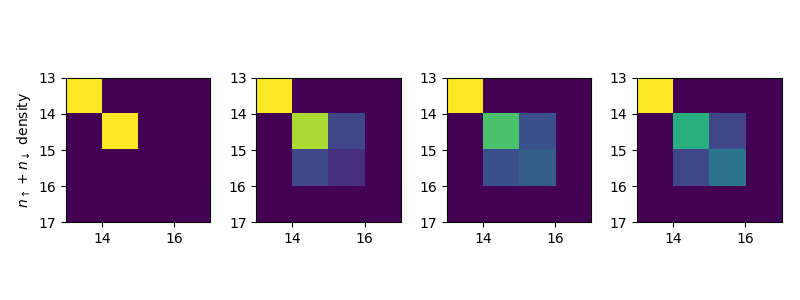
\includegraphics[width=0.5\textwidth]{images/vmc_2orb_obdm.png}
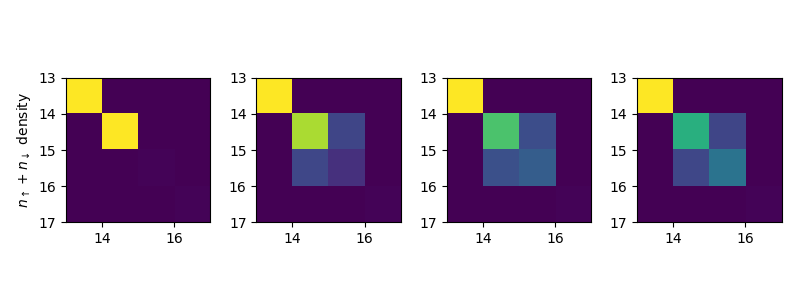
\includegraphics[width=0.5\textwidth]{images/dmc_2orb_obdm.png}
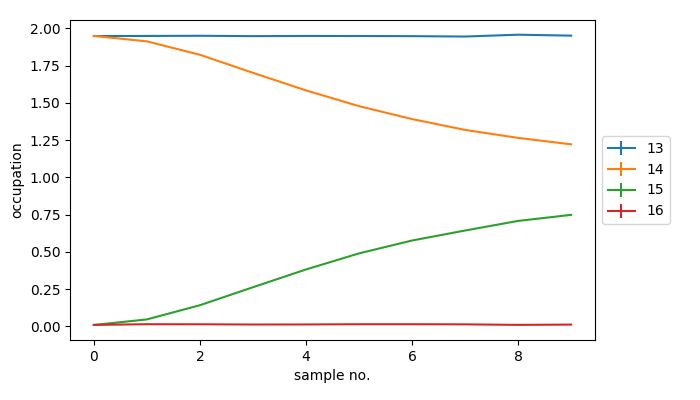
\includegraphics[width=0.5\textwidth]{images/vmc_2orb_occupations.png}
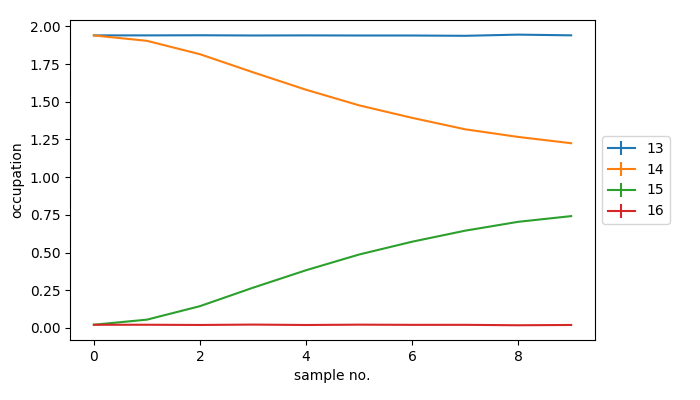
\includegraphics[width=0.5\textwidth]{images/dmc_2orb_occupations.png}
\caption{
Left: VMC; Right: DMC. 
(Top) Part of the one-body density matrix computed from different wave functions, showing the matrix elements that change across samples. 
(Bottom) The orbital occupations (diagonal of OBDM) plotted against determinant weight $c_1$.
}
\label{fig:obdm}
\end{figure}

\noindent {\bf Descriptors }

Only the occupations of orbitals 16 and 17 change noticeably across samples.
The two determinants have either orbital 16 or 17 occupied, and all other occupations are the same, so this is not surprising, and the population of orbital 17 increases with the weight of determinant $S_1$.
This tells us only orbitals 16 and 17 can be relevant to the model.
Since the trace of the OBDM is the number of electrons ($n_{16}+n_{17}=2$), there is only one degree of freedom, which we choose to be $n_{17}$.

\noindent {\bf Fitting a model }

The model is 
\begin{equation}
\expectation{H} = E = \epsilon_0 + \epsilon_{17} \expectation{\hat{n}_{17}},
\label{eq:2orb_model}
\end{equation}

with a constant energy shift $\epsilon_0$ and a term proportional to $n_{17}$, the occupation of orbital 17, with coefficient $\epsilon_{17}$, which should be the energy of the one-particle excitation.
Using least squares regression, we compute $\epsilon_0$ and $\epsilon_{17}$, and compare the fit to the data points from VMC. 
The computed values are 

\begin{tabular}{c|cc}
 & $\epsilon_0$ & $\epsilon_{17}$ \\\hline
VMC & -31.073 & .0871 \\
DMC & -31.279 & .0428
\end{tabular}

\begin{figure}
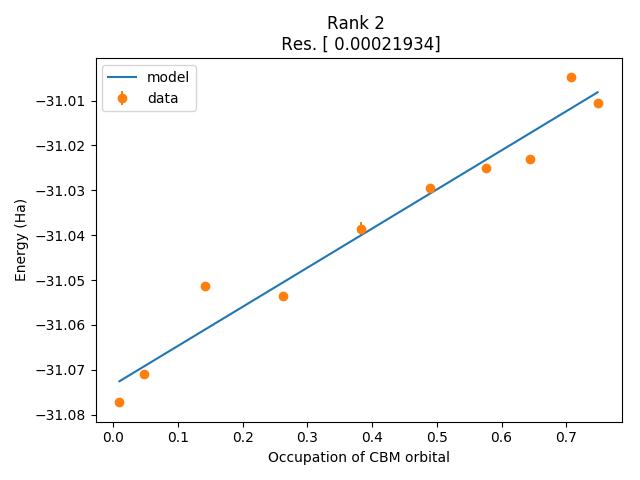
\includegraphics[width=0.5\textwidth]{images/vmc_2orb_model.png}
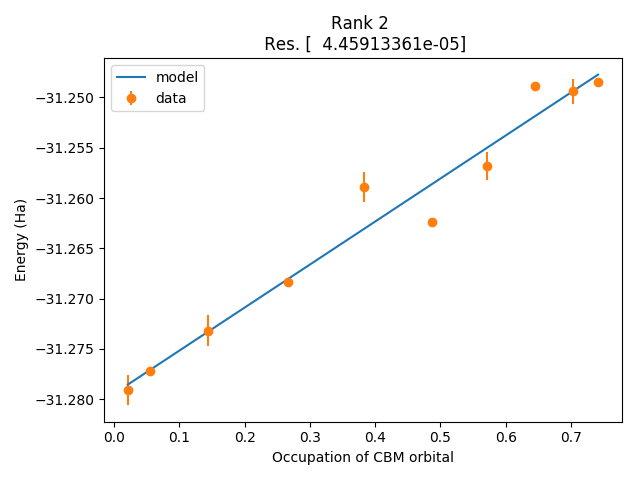
\includegraphics[width=0.5\textwidth]{images/dmc_2orb_model.png}
\caption{
Left: VMC; Right: DMC. 
Energy vs occupation $n_{17}$. The line is the linear fit, the points are from simulation (with error bars in both energy and density).
}
\label{fig:2orb_model}
\end{figure}

\subsection{Parameter derivatives}

The samples used to fit the model above (Eq \ref{eq:2orb_model}) depend on the parameter $c_{1}$ ($c_{0}$ is set by normalization).

Differentiating the model (Eq \ref{eq:2orb_model}) with respect to the determinant weight $c_1$  yields another equation with the model parameter $\epsilon_{17}$,

\begin{equation}
\frac{\partial E}{\partial c_1} = \epsilon_{17} \frac{\partial n_{17}}{\partial c_1}.
\label{eq:2orb_deriv}
\end{equation}

We compute this derivative and include the additional equations in the model fitting (note that the constant shift $\epsilon_0$ doesn't appear in the derivative equation).

\begin{figure}[h]
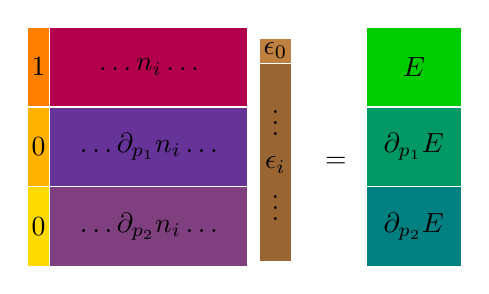
\begin{tikzpicture}[const/.style={rectangle, minimum height=1cm, inner sep=.5mm},
                    occ/.style={rectangle, minimum height=1cm, minimum width=2.5cm},
                    en/.style={rectangle, minimum height=1cm, minimum width=1.2cm}]
\node (1) [const, fill=orange] {1};
\node (01) [const, below=0mm of 1.south east, anchor=north east, fill=orange!60!yellow] {0};
\node (02) [const, below=0mm of 01.south east, anchor=north east, fill=orange!30!yellow] {0};
\node (n) [occ, right=0mm of 1.south east, anchor=south west, fill=red!70!blue] {$\ldots n_i \ldots$};
\node (n1) [occ, right=0mm of 01.south east, anchor=south west, fill=blue!60!orange] {$\ldots \partial_{p_1} n_i \ldots$};
\node (n2) [occ, right=0mm of 02.south east, anchor=south west, fill=blue!50!orange] {$\ldots \partial_{p_2} n_i \ldots$};
\node (param0) [rectangle, below right=2mm of n.north east, anchor=north west, fill=brown!100!red, minimum width=4mm, inner sep=.5mm] {$\epsilon_0$};
\node (params) [rectangle, below=0mm of param0, anchor=north, fill=brown!80!black, minimum height=2.5cm, minimum width=4mm, inner sep=.5mm] 
{$\begin{matrix} \vdots\\ \epsilon_i\\ \vdots \end{matrix}$};
\node (=) [right=3mm of params] {$=$};
\node (E) [en, right=15mm of n.north east, anchor=north west, fill=green!80!black] {$E$};
\node (E1) [en, below=0mm of E.south, anchor=north, fill=green!60!blue] {$\partial_{p_1} E$};
\node (E2) [en, below=0mm of E1.south, anchor=north, fill=green!50!blue] {$\partial_{p_2} E$};
\end{tikzpicture}
\end{figure}


\begin{figure}
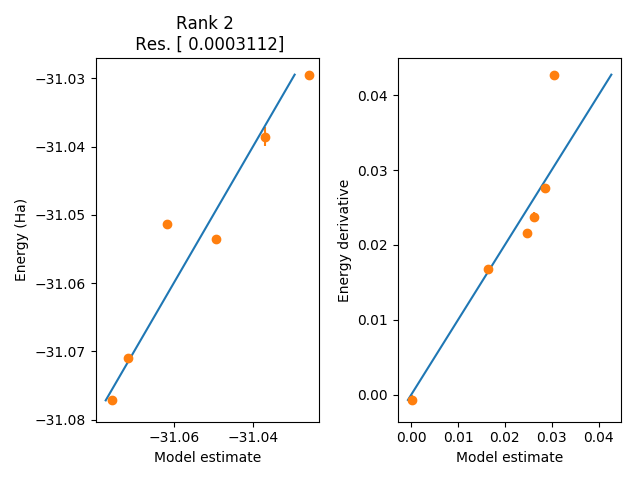
\includegraphics[width=0.5\textwidth]{images/vmc_allderivs_2orb_model.png}
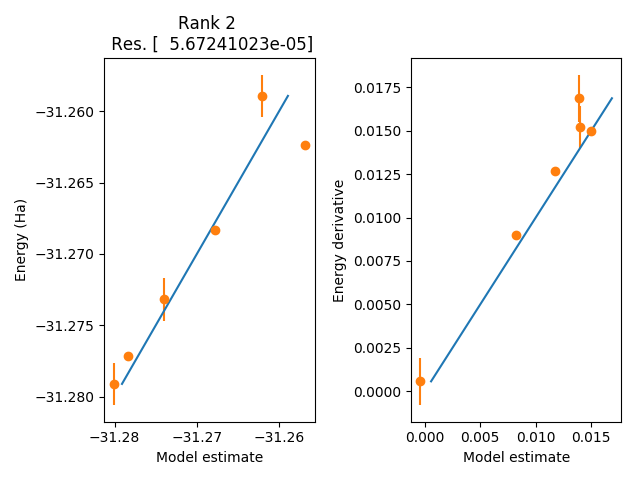
\includegraphics[width=0.5\textwidth]{images/dmc_allderivs_2orb_model.png}
\label{fig:2orb_deriv}
\caption{
Left: VMC; Right: DMC.
In the left panel, the fit is shown for the energies; in the right panel, it is shown for the energy derivatives.
(The parameter $\epsilon_17$ is computed using all the equations together.)}
\end{figure}

The computed values using the parameter derivative are 

\begin{tabular}{c|cc}
 & $\epsilon_{0}$ & $\epsilon_{17}$ \\\hline
VMC & -31.076 & 0.1034 \\
DMC & -31.281 & 0.0500 
\end{tabular}



\section {Low energy states}

Including more states and more derivatives allows us to use better statistics and fit more complicated models.
To describe the low energy degrees of freedom, we choose determinants corresponding to low energy mean-field excitations.

\subsection{Choosing excitations}

\begin{figure}[h!]
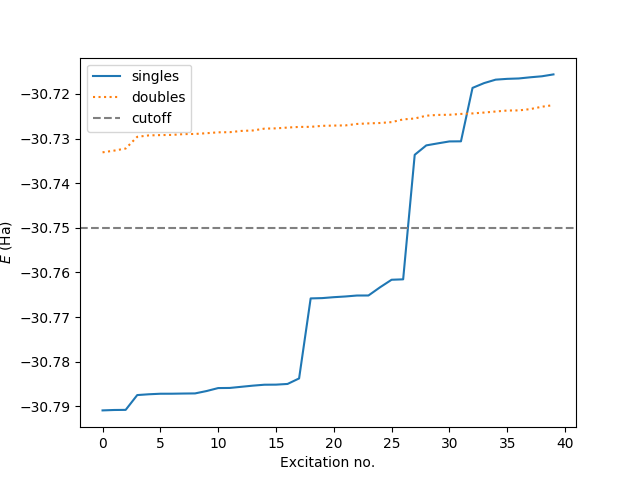
\includegraphics[width=0.5\textwidth]{images/determinant_mf_energies.png}
\label{fig:energy_cutoff}
\caption{Mean-field DFT energies for singles and doubles excitations.
The dashed line shows the cutoff chosen for the samples used in this calculation.}
\end{figure}

To fit a ``low energy'' model, it is ideal to choose states below an energy gap so that the states are well described by the low energy subspace of the Hilbert space.
(If there is no gap, the states may have components not included in the low energy space, introducing energy variance that is not relevant to the model.)
We choose an energy cutoff in the gap shown in Fig \ref{fig:energy_cutoff}, which only includes singles excitations.

\subsection{Wave function samples}

As with the model above, the model we are fitting here assigns new energies to the molecular orbitals,

\begin{equation}
E = \epsilon_0 + \sum_i \epsilon_i n_i,
\end{equation}

where $i$ indexes a set of molecular orbitals.
In this set of samples, a total of 12 orbitals have varying occupation (three valence, nine conduction, Fig \ref{fig:descriptors}).
Since the total number of electrons is constant, there are only 11 degrees of freedom in the orbital occupations.

\begin{figure}[h!]
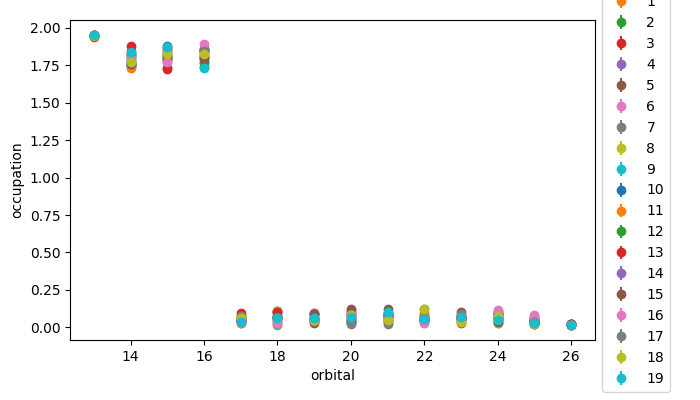
\includegraphics[width=0.5\textwidth]{images/vmc_lowen_descriptors.png}
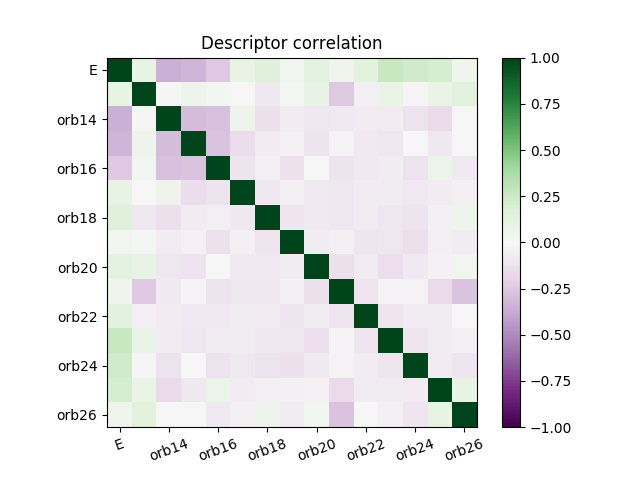
\includegraphics[width=0.5\textwidth]{images/vmc_allderivs_lowen_corrmat.png}
\label{fig:descriptors}
\caption{Left: Occupation of orbitals for different samples. Right: The correlation matrix (VMC) of the energies and orbital occupations, including derivatives.}
\end{figure}

The correlation matrix of the descriptors shows how the energy is correlated with the orbital occupations (Fig \ref{fig:descriptors}).
The correlation samples include both the values and derivatives of the energies and occupations.
Since there is a constant term in the model, the mean of the energies was subtracted off (but not of the derivatives).
As we should expect, the energy is negatively correlated with the valence occupations, and positively correlated with the conduction occupations.

Unfortunately, this trend is not present without the derivatives
\begin{figure}[h!]
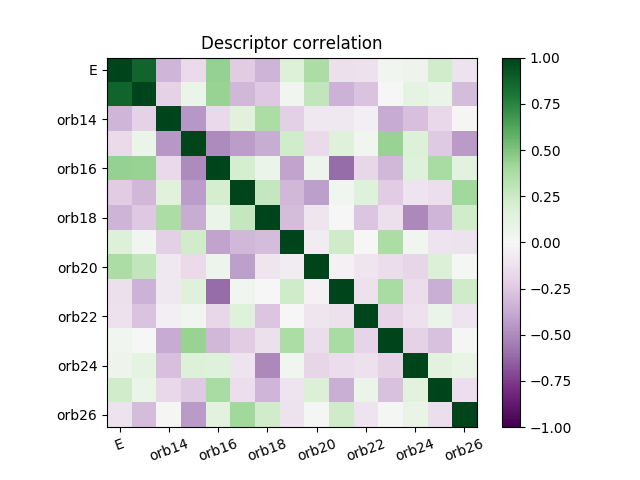
\includegraphics[width=0.5\textwidth]{images/vmc_lowen_corrmat.png}
\label{fig:descriptors_noderivs}
\caption{The correlation matrix (VMC) of the energies and orbital occupations (not including derivatives).}
\end{figure}

\subsection{Fitting a model}

Two models are fit: one using only the energies and occupations, the other also using the derivatives.
There seems to be an issue with the energies, but the derivatives seem to fit well.

\begin{figure}[h!]
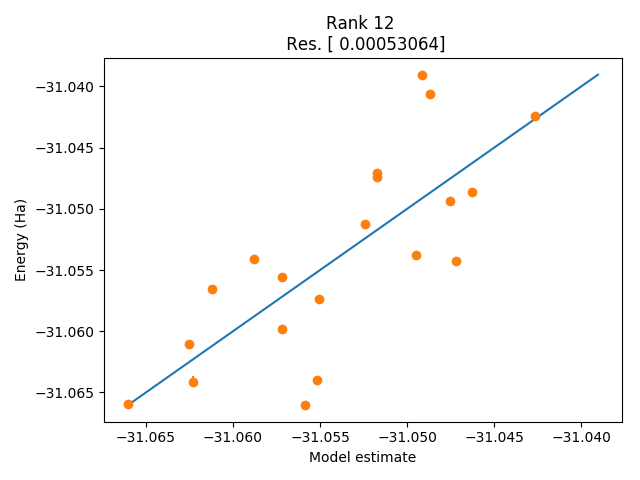
\includegraphics[width=0.5\textwidth]{images/vmc_lowen_model.png}
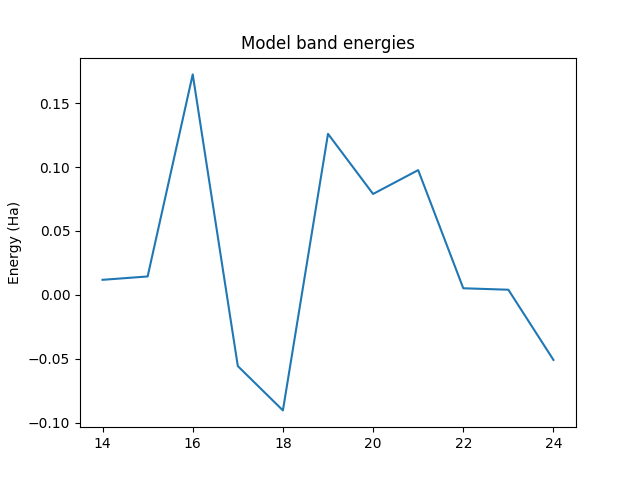
\includegraphics[width=0.5\textwidth]{images/vmc_lowen_model_bands.png}
\label{fig:model_fit_noderivs}
\caption{Model fit without derivatives. Left: Plot of data vs model prediction. Right: The orbital energies of the model.}
\end{figure}

\begin{figure}[h!]
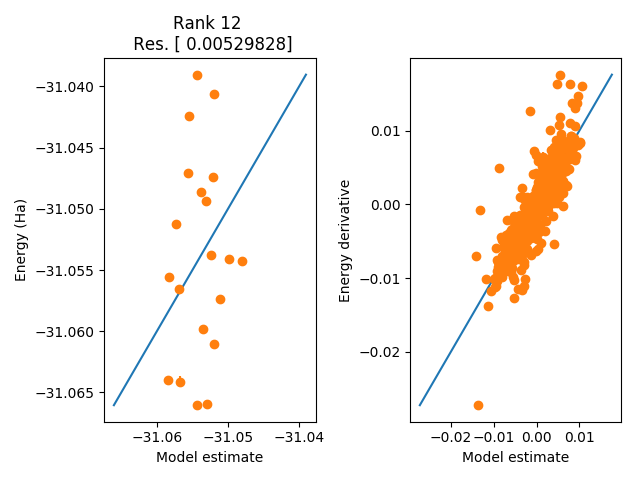
\includegraphics[width=0.5\textwidth]{images/vmc_allderivs_lowen_model.png}
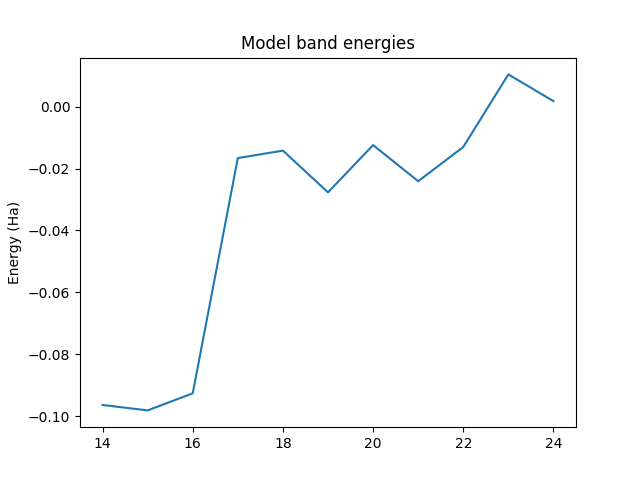
\includegraphics[width=0.5\textwidth]{images/vmc_allderivs_lowen_model_bands.png}
\label{fig:model_fit}
\caption{Model fit with derivatives. Left: Plot of data vs model prediction. Right: The orbital energies of the model.}
\end{figure}

  
  




\end{document}
